\setcounter{exo}{0}


\begin{center}
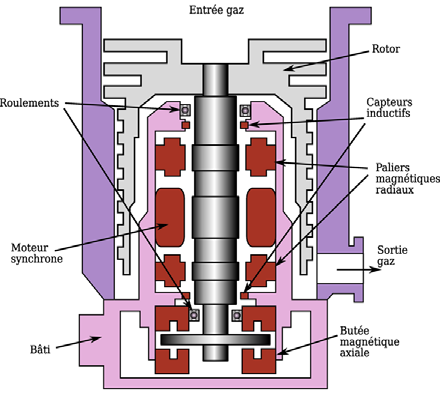
\includegraphics[width=.9\linewidth]{fig_05}
\end{center}

\setcounter{exo}{0}
On considère un bâti \textbf{0} auquel est attaché le repère$\mathcal{R}=\left(O;\vect{x_0};\vect{y_0};\vect{z_0} \right)$. Le champ de pesanteur est $g=-g\vect{y_0}$.La barre \textbf{1} est liée au bâti \textbf{0} par une liaison pivot parfaite d’axe $\left(A,\vect{z_0}\right)$. Le plateau porte camion \textbf{2} est lié à la barre \textbf{1} par une liaison pivot parfaite d’axe $\left(C,\vect{z_0}\right)$. Le levier \textbf{3} est lié au bâti \textbf{0} par une liaison pivot parfaite d’axe $\left(B,\vect{z_0}\right)$. Ce levier est également lié au plateau \textbf{2} par une liaison pivot parfaite d’axe $\left(D,\vect{z_0}\right)$. Le camion \textbf{4}, de centre de masse $G$ et de masse $M$ inconnue, repose sur le plateau \textbf{2}.
L’action mécanique connue est caractérisée par : $\{\text{ext}\rightarrow 3\}=\left\{
\begin{array}{c}
-F\vect{y_0} \\
\vect{0} \\
\end{array}
\right\}_E$ .




\subparagraph{}\textit{Tracer le graphe de structure. Définir le nombre d'inconnues statiques.}

\subparagraph{}\textit{Donner la stratégie permettant de déterminer la valeur de $F$ en fonction de $M$.}

\subparagraph{}\textit{Déterminer la relation entre $F$ et $M$. Que dire de la position du camion sur la plate-forme ?}

\subparagraph{}\textit{Déterminer les actions mécaniques dans toutes les liaisons.}
